\documentclass{beamer}
%
% Choose how your presentation looks.
%
% For more themes, color themes and font themes, see:
% http://deic.uab.es/~iblanes/beamer_gallery/index_by_theme.html
%
\mode<presentation>
{
  \usetheme{default}      % or try Darmstadt, Madrid, Warsaw, ...
  \usecolortheme{default} % or try albatross, beaver, crane, ...
  \usefonttheme{default}  % or try serif, structurebold, ...
  \setbeamertemplate{navigation symbols}{}
  \setbeamertemplate{caption}[numbered]
}

\usepackage[english]{babel}
\usepackage[utf8]{inputenc}
\usepackage[T1]{fontenc}
\usepackage[]{graphicx}
\usepackage{caption}
\usepackage{subcaption}

\newcommand{\emphbf}[1]{\textbf{\emph{#1}}}

\title[Graphics Pipeline]{The Real-Time Graphics Pipeline}
\author{Benjamin Brown}
%\institute{Where You're From}
\date{Monday, 26th September 2022}

\begin{document}

\begin{frame}
  \titlepage
\end{frame}

% Uncomment these lines for an automatically generated outline.
%\begin{frame}{Outline}
%  \tableofcontents
%\end{frame}

\begin{frame}{The Key Idea}

Aim is to \emphbf{render} 3d objects on 2d screen

\vskip 1cm

Two methods of rendering:

\begin{itemize}
	\item \emphbf{object-order rendering}: for each \textcolor{blue}{object}, which \textcolor{red}{pixels} are influenced by it?
	\item \emphbf{image-order rendering}: for each \textcolor{red}{pixel}, which \textcolor{blue}{object} is influenced by it?
\end{itemize}

\end{frame}

\begin{frame}{Object- vs. Image-Order Rendering}

	\begin{figure}
		\centering
		\begin{minipage}{.5\textwidth}
			\centering
			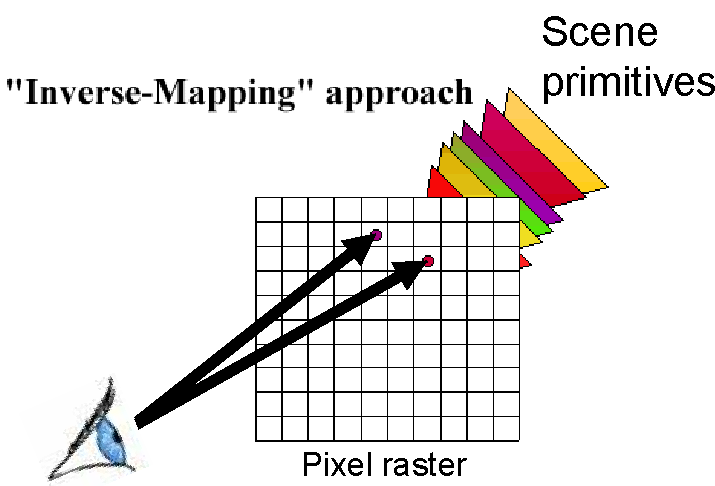
\includegraphics[width=.8\linewidth]{image-order}
			\caption{Image-order rendering.}
		\end{minipage}%
		\begin{minipage}{.5\textwidth}
			\centering
			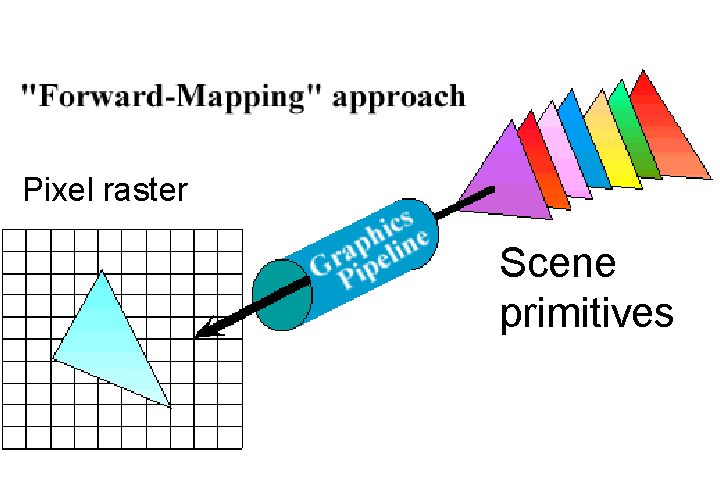
\includegraphics[width=.8\linewidth]{object-order}
			\caption{Object-order rendering.}
		\end{minipage}
	\end{figure}

\end{frame}

\begin{frame}{Real-Time Rendering}

	\emphbf{Real-time} refers to rendering a scene in less than 1/30\textsuperscript{th} of a second.

	\begin{itemize}
		\item Fast enough to allow for the user's \emphbf{real-time interaction}.
		\item Temporal delay of 15 ms of temporal delay can interfere with the interactivity.
	\end{itemize}

	\vskip 1cm

	Speed is essential!

	\begin{itemize}
		\item 1080p image at 90 Hz, image-order rendering needs 186,624,000 iterations times per second!
	\end{itemize}

\end{frame}

\begin{frame}{The Graphics Pipeline}

	Object-order rendering uses the \emphbf{graphics pipeline}:

	\begin{itemize}
		\item Given a virtual camera, 3d objects, light sources, etc., render a 2d image;
		\item Object locations and shapes determined by their geometry, environment,  camera placement, etc.;
		\item Object appearance affected by material, light sources, shading, etc.
	\end{itemize}

	\vskip 1cm

	The states execute in parallel; each stage depends on the previous.

\end{frame}

\begin{frame}{Stages of the Graphics Pipeline}

	Roughly, these stages are:

	\vskip 1cm

	\begin{figure}[t]
		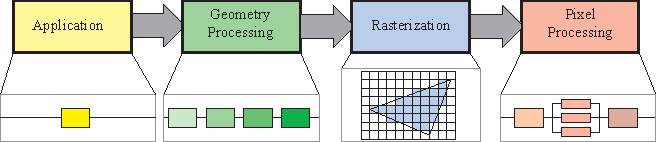
\includegraphics[width=10cm]{main-pipeline}
		\centering
	\end{figure}

	\vskip 1cm

	Geometry processing, rasterisation, and pixel processing happen within the \emphbf{GPU}.

\end{frame}

\begin{frame}{Stages of the Graphics Pipeline}

	\begin{figure}[t]
		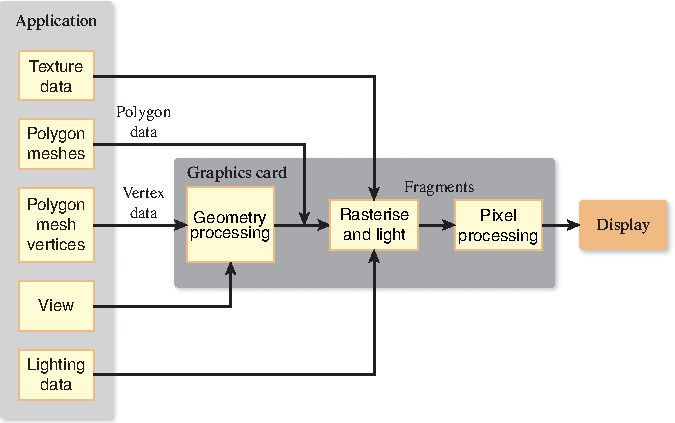
\includegraphics[width=10cm]{pipeline-2}
		\centering
	\end{figure}

\end{frame}

\begin{frame}{Application Stage}

	The \emphbf{application} on the \emphbf{CPU} supplies the data about the scene to the \emphbf{GPU}:

	\vskip 1cm

	\begin{itemize}
		\item \emphbf{Primitive} data:
		\begin{itemize}
			\item Vertex data (position, normal vectors, colour, etc.),
		\end{itemize}
		\item Initialises GPU memory \emphbf{buffers}:
		\begin{itemize}
			\item Vertex and index buffers.
		\end{itemize}
	\end{itemize}

\end{frame}

\begin{frame}{Geometry Processing Stage}

	Performs per-triangle and per-vertex operations:

	\begin{itemize}
		\item Vertex processing (transforming and shading);
		\item Projecting;
		\item Clipping;
		\item Screen mapping.
	\end{itemize}

	\vskip 1cm

	\begin{figure}[t]
		
\includegraphics[width=10cm]{geometry-pipeline}
		\centering
	\end{figure}

\end{frame}

\begin{frame}{The Geometry Stage -- Transformations}

	\begin{figure}[t]
		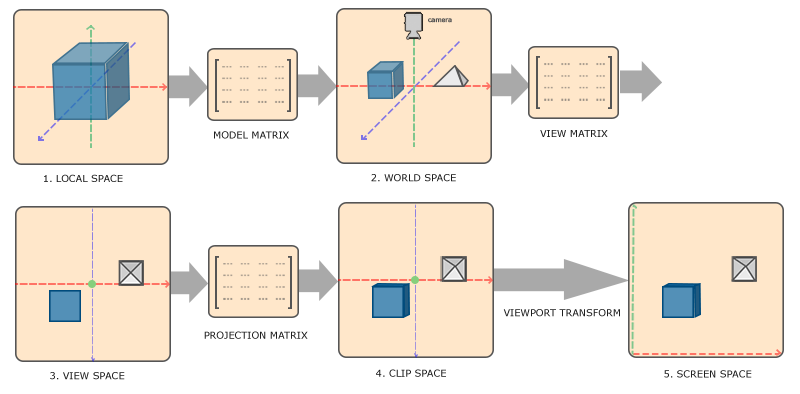
\includegraphics[width=11cm]{coordinate-systems}
		\centering
	\end{figure}

\end{frame}

\begin{frame}{The Geometry Stage -- Local-to-View Space}

	\begin{figure}[t]
		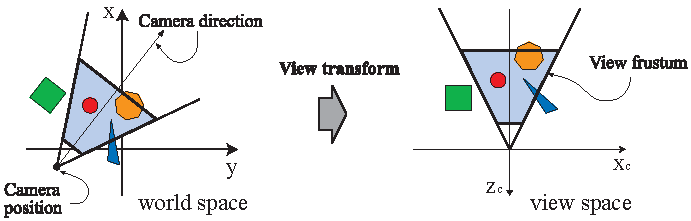
\includegraphics[width=11cm]{view-transform}
		\centering
	\end{figure}

\end{frame}

\begin{frame}{The Geometry Stage -- Vertex Shading}

	\begin{figure}[t]
		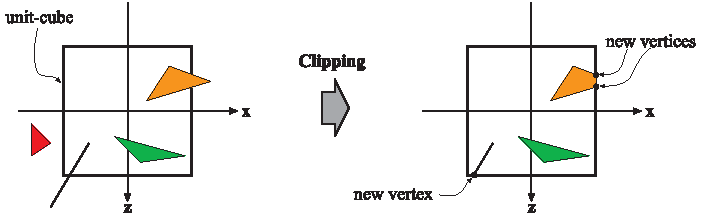
\includegraphics[width=11cm]{clipping}
		\centering
	\end{figure}

\end{frame}

%\begin{frame}{Geometry Processing Stage -- Vertex Processing}
%
%	\emphbf{Vertex shading} deals with:
%
%	\begin{itemize}
%		\item Determining the effect of a light on a material (\emphbf{shading});
%		\item Projecting from \emphbf{world space} onto \emphbf{view space};
%		\item \emphbf{Clipping} away the view space primitives which do not lie within the view volume;
%		\item Mapping the vertices onto \emphbf{screen space};
%	\end{itemize}
%
%\end{frame}

\begin{frame}{The Rasterisation Stage}

	\emphbf{Rasterisation} can be split into two sub-pipelines:

	\begin{figure}[t]
		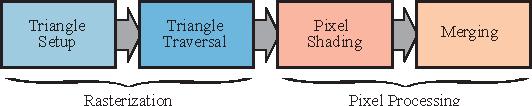
\includegraphics[width=8cm]{rasterisation-pipeline}
		\centering
	\end{figure}

	\begin{figure}[t]
		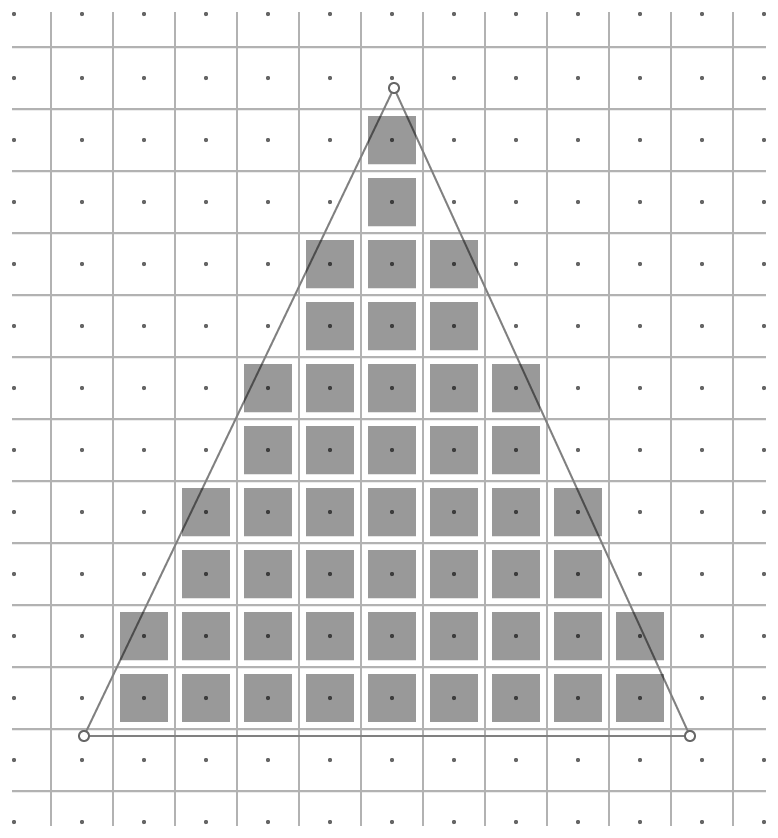
\includegraphics[height=4cm]{fragment}
		\centering
	\end{figure}

	Data for each pixel is called a \emphbf{fragment}.

\end{frame}

\begin{frame}{The Rasterisation Stage -- Pixel Shading}

	\begin{itemize}
		\item Example -- fragment data from interpolation.
	\end{itemize}

%	\vskip 1cm

	\begin{figure}
		\centering
		\begin{minipage}{.35\textwidth}
			\centering
			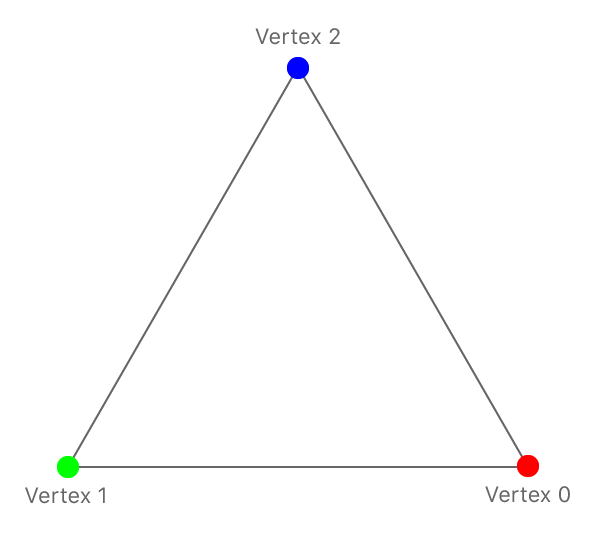
\includegraphics[width=.8\linewidth]{triangle}
%			\caption{Vertex colour values.}
		\end{minipage}%
		$\longmapsto$
		\begin{minipage}{.35\textwidth}
			\centering
			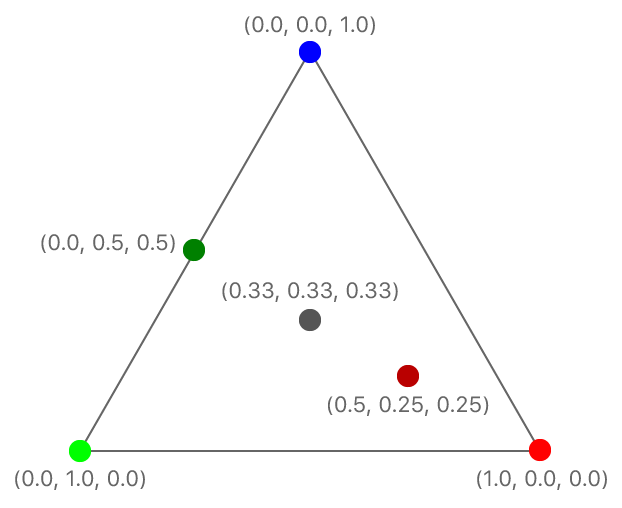
\includegraphics[width=.8\linewidth]{interpolation}
%			\caption{Interpolated fragment colour values.}
		\end{minipage}
	\end{figure}

	\begin{figure}[t]
		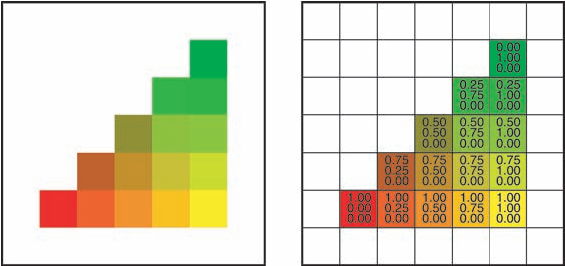
\includegraphics[height=3cm]{interpolation-2}
		\centering
	\end{figure}

\end{frame}

\begin{frame}{The Rasterisation Stage -- Pixel Shading}

	\begin{itemize}
		\item Example -- light shading.
	\end{itemize}

	\vskip 1cm

	\begin{figure}
		\centering
		\begin{minipage}{.5\textwidth}
			\centering
			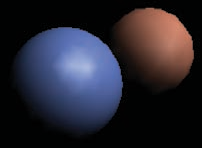
\includegraphics[width=.8\linewidth]{shading-1}
			\caption{Per-vertex shading.}
		\end{minipage}%
		\begin{minipage}{.5\textwidth}
			\centering
			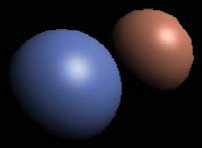
\includegraphics[width=.8\linewidth]{shading-2}
			\caption{Per-fragment shading.}
		\end{minipage}
	\end{figure}

\end{frame}

\begin{frame}{The Rasterisation Stage -- Pixel Shading}

	\begin{itemize}
		\item Example -- texture mapping.
	\end{itemize}

	\vskip 1cm

	\begin{figure}[t]
		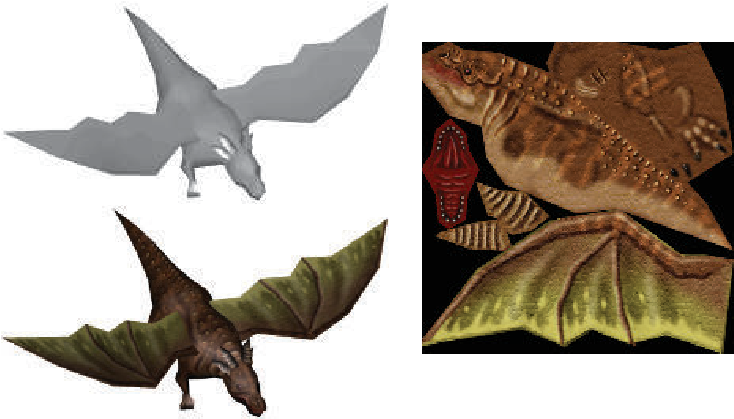
\includegraphics[height=6cm]{texture-mapping}
		\centering
	\end{figure}

\end{frame}

\begin{frame}{The Rasterisation Stage -- Merging}

	\begin{itemize}
		\item Storing pixels in a colour buffer;
		\item With a depth- or $z$-buffer.
	\end{itemize}

%	\vskip 1cm

	\begin{figure}
		\centering
		\begin{minipage}{.5\textwidth}
			\centering
			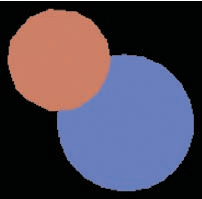
\includegraphics[width=.8\linewidth]{depth-1}
			\caption{No depth sorting.}
		\end{minipage}%
		\begin{minipage}{.5\textwidth}
			\centering
			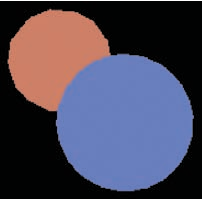
\includegraphics[width=.8\linewidth]{depth-2}
			\caption{With depth sorting.}
		\end{minipage}
	\end{figure}

\end{frame}


\begin{frame}{Final Remarks}

	Modern day 3d graphics APIs include:

	\begin{itemize}
		\item Vulkan/OpenGL (Khronos Group);
		\item Direct3D (Microsoft);
		\item Metal (Apple).
	\end{itemize}

	\vskip 1cm

	The pipeline performs parallel and regular computations $\implies$ GPUs are specialised for this!

\end{frame}

\end{document}
